\documentclass{article}

% Essential packages
\usepackage{graphicx}   % For image handling
\usepackage{subcaption} % For multi images
\usepackage{caption}    % For proper captions
\usepackage{listings}   % For code listings
\usepackage{fontspec}   % For custom fonts
\usepackage{xcolor}     % For color support
\usepackage{tcolorbox}  % For code block boxes
\usepackage{etoolbox}   % For patching and command manipulation
\usepackage{titlesec}   % For section formatting
\usepackage{parskip}    % For customisable paragraph formating
\usepackage{comment}    % For being able to comment out sections
\usepackage{geometry}   % For managing page size and margins
\usepackage{hyperref}   % For embedding links, like URL's

\tcbuselibrary{listings, skins, breakable}  %Librarary to make code blocks multipage


%   ############################## Customisation ##############################

% Document metadata
\title{\fontsize{24}{36}\selectfont This is the title of the\\ %Edit title here \\ means new line
document} % Line 2 of title, its not subtitle, that is possible to, google it
\author{Your Name} % Input your name
\date{\today} % Auto updates the date, untill you export it, replace with hardcoded date if you need

% Adjust the body text font size to 12pt without affecting section headings
\renewcommand{\normalsize}{\fontsize{12}{16}\selectfont}

% Adjust the paragraph spacing, either as indentation or/and line spaceing
\setlength{\parindent}{0pt}  % Remove indentation
\setlength{\parskip}{6pt}    % Add vertical space between paragraphs

% Customisation of fonts and colors
\setmainfont{Times New Roman}
\setmonofont{JetBrains Mono}
\definecolor{background}{RGB}{225, 219, 202}
\definecolor{darkAccent}{RGB}{140, 98, 64}
\definecolor{commentGreen}{RGB}{26, 159, 32}
\definecolor{keywordPurple}{RGB}{229, 24, 192}
\definecolor{keywordBlue}{RGB}{5, 142, 217}
\definecolor{portOrange}{RGB}{234, 72, 31}
\definecolor{darkGray}{RGB}{60, 60, 60}

% Link color customization
\hypersetup{
    colorlinks=true,
    linkcolor=darkGray, % Internal links such as table of contents or figure referencing
    urlcolor=keywordBlue % URL colors
    }
\urlstyle{same} % Makes url in the same style as the rest of the document

% Customisation of margins and paper size
\geometry{
 a4paper,
 left = 30mm,
 right = 30mm,
 top = 30mm,
 bottom = 30mm
 }

% Sections formatting and numbering
% Sets the font to monospace for section, subsection and subsubsection
% and sets the format to be numbers with . between and at the end
\renewcommand{\thesection}{\texttt{\arabic{section}.}}
\renewcommand{\thesubsection}{\texttt{\arabic{section}.\arabic{subsection}.}}
\renewcommand{\thesubsubsection}{\texttt{\arabic{section}.\arabic{subsection}.\arabic{subsubsection}.}}

\setcounter{section}{-1}  % Start section numbering from 0, delete this to start from 1

% Makes section monospace font and start each subsection from 0
\let\oldsection\section
\renewcommand{\section}[1]{%
  \oldsection{\texttt{#1}} % Make section title monospace
  \setcounter{subsection}{-1} % Makes subsection start from 0, delete this line to start from 1
  \setcounter{figure}{-1} % Makes figure numbers start from 0, delete this line to start from 1
}

% Makes subsection monospace font and start each subsubsection from 0
\let\oldsubsection\subsection
\renewcommand{\subsection}[1]{%
  \oldsubsection{\texttt{#1}}% Make subsection title monospace
  \setcounter{subsubsection}{-1}% Makes subsubsection start from 0, delete this line to start from 1
}

% Makes subsubsection monospace font
\let\oldsubsubsection\subsubsection
\renewcommand{\subsubsection}[1]{%
  \oldsubsubsection{\texttt{#1}}% Make subsubsection title monospace
}

% Makes every new section start on a new page, except for the first section, section 0
\pretocmd{\section}{%
  \ifnum\value{section}=-1 \else\clearpage\fi % Replace -1 with 0 if sections start at nr. 1
}{}{}

% Makes Table of contents a subsection
\makeatletter
\renewcommand{\tableofcontents}{%
    \subsection{Table of Contents} % Numbered subsection named Table of contents
    \@starttoc{toc}%
}
\makeatother

% Makes List of figures a subsection
\makeatletter
\renewcommand{\listoffigures}{%
    \subsection{List of Figures} % Numbered subsection named List of figures
    \@starttoc{lof}%
}
\makeatother

% Makes every figure be formated as section number.figure number
\renewcommand{\thefigure}{\arabic{section}.\arabic{figure}}

% Add keywords to be highlited in blue below. Note that all reserved
% keywords from VHDL is already in purple and should not be added here
% too as duplicates will cause issues. Therfore compile this document
% after pasting in code and only add non-highlited words to this list.
% Also, there is not a list for orange keywords, used for ports here.
\lstdefinelanguage{VHDL+}{
    language     = VHDL,
    morestring = [b]',
    morekeywords = [2]{
        IEEE,
        std_logic_1164, std_logic, std_logic_vector},
    morekeywords = [3]{
        SW, LEDR, KEY,
        HEX0, HEX1, HEX2, HEX3, HEX4, HEX5, HEX6},
    sensitive = false
}


%   ############################## Advanced customisation ##############################

% Customisation of list style inside code block
\lstdefinestyle{VHDL}{
    language = VHDL+, % Uses the extra higlights from above
    % The folloowing lines defines color for highlighting, other changes like
    % italic, bold or different fonts can also be added to this
    commentstyle = \color{commentGreen}, 
    keywordstyle = \color{keywordPurple},
    keywordstyle = [2]\color{keywordBlue},
    keywordstyle = [3]\color{portOrange},
    stringstyle = \color{darkAccent},
    basicstyle = \ttfamily\small, % Default font inside code block
    numberstyle = \ttfamily\color{darkAccent}, % Style of line numbering
    numbers = left, % Line numbering on left side
    breakatwhitespace = false, % Don't start new line with only whitspaces
    breaklines = true, % If line is to long it will wrap to next line (line number does not increase)
    keepspaces = true, % Indents works logical
    showspaces = false, % Space is blank character, set to true to show dots instad
    showstringspaces = false, % Same as above but inside strings
    showtabs = false, % Tab is also blank character, set to true to show dashes
    tabsize = 4, % Tabsize is set to 4, this works well with code from notepad++
    % Dont mess with the ones below unless you want to mess with the box as well
    % These took some time to line up such that it looks natural
    numbersep = 10pt, % Adjust distance between numbers and code
    xleftmargin = -8pt,% Negative margin to pull code text closer to the left border
}

% This is for code where VHDL is not an argument
\lstdefinestyle{Example Code}{
    basicstyle = \ttfamily\small, % Default font inside code block
    numberstyle = \ttfamily\color{darkAccent}, % Style of line numbering
    numbers = left, % Line numbering on left side
    breakatwhitespace = false, % Don't start new line with only whitspaces
    breaklines = true, % If line is to long it will wrap to next line (line number does not increase)
    keepspaces = true, % Indents works logical
    showspaces = false, % Space is blank character, set to true to show dots instad
    showstringspaces = false, % Same as above but inside strings
    showtabs = false, % Tab is also blank character, set to true to show dashes
    tabsize = 4, % Tabsize is set to 4, this works well with code from notepad++
    % Dont mess with the ones below unless you want to mess with the box as well
    % These took some time to line up such that it looks natural
    numbersep = 10pt, % Adjust distance between numbers and code
    xleftmargin = -8pt,% Negative margin to pull code text closer to the left border
}

\lstset{style = Example Code} %Sets the default style to Example Code

% Customisation of code block itself
\newtcolorbox[auto counter, number within=section]{codeBlock}[2][]{
    colback=background, % Background color for the code block
    colframe=darkAccent, % Border color for the code block
    listing only, %Makes it contain the listing
    arc=10pt, % Rounded corners size
    sharp corners=northeast, % Make top-right corner sharp for the main box
    enhanced jigsaw, % Essential dont mess with it
    breakable, % Allows content to be multipage
    top=-4pt, % Made to line up text dont mess with it
    bottom=-4pt, % Same as above
    before skip=0pt, after skip=10pt, % Adjust spacing before and after the box
    boxrule=1pt, % Border thickness of the main box
    overlay unbroken and first={\node[ % Create label box in the top-right corner
        anchor=north east,      %Position of box, same as sharp corner in this case
        fill=background,        %Background color same as main box
        draw=darkAccent,        %Outline color, same as main box
        line width=1pt,         %Outline thickness, same as main box
        text=keywordPurple,     %Text color
        font=\ttfamily,         %Text font and size
        inner sep=6pt,          %Spacing inside
        minimum width=16pt,     %Minimum box with, it autoresizes depending on text
        minimum height=12pt,    %Minimum box height, it autoresizes depending on text
        text centered,          %Centres the text with the spacing
        sharp corners]          %Makes corners sharp
        at ([xshift=0pt, yshift=0pt]frame.north east) % Position, aligned with corner on main box
        {#2}; % Types your argument in the top corner as a label
    }
}

% This is the custom command used for inserting code blocks
\newcommand{\writecode}[3][Example Code]{%
    \begin{codeBlock}{#1}% arg 1 (default Example Code) will be writtin in top right corner box
        \lstinputlisting[style=#1]{Code/#2}% arg 1 style is used and arg 2 is filename
    \end{codeBlock}%
    \begin{figure}[h] % Empty figure for captioning and referencing
        \centering
        \renewcommand\figurename{Code}
        %\captionsetup{type=figure, name=Code}
        \caption{#3} % arg 3 is used for caption
        \label{Code:#2} % Uniqe label for referencing is using file name
    \end{figure}
}

% This is the custom command used for making the introduction section
\newcommand{\introduction}[1][]{%
    \addtocontents{toc}{\protect\setcounter{tocdepth}{0}} % Temporarily hide from TOC
    \section{Introduction} % Numbered section named Introduction
    \ifx\relax#1\relax % Check if argument is empty
    \else
        #1 % Insert the optional text if provided
    \fi
    \tableofcontents % Generate TOC
    \clearpage
    \listoffigures % List of figures
    \addtocontents{toc}{\protect\setcounter{tocdepth}{2}} % Restore TOC depth
}



%   ############################## Document begins here ##############################

\begin{document}

\maketitle % Makes title front page based on the title, author and date metadata, change at the top


%           ########## Section ##########
% This makes the first section, introduction, that are excluded from the table of contents and
% has an optional text argument, then it creates table of contents and list of figures
\introduction[
This is a template. Note: The \LaTeX\ code is open source, \href{https://github.com/Kjelseth/PLK_lab.git}{github link}.
]


%   ############################## Section ##############################
\section{Section on inserting}
This task was a introductory task...

\subsection{Code}
\writecode[VHDL]{Example1.vhd}{Example of code inserting} % This is how to add code block
% syntax is \writecode[language]{filename}{Caption}
% the three arguments are [optional]{mandatory}{mandatory}
% [language] is the optional argument for code language, currently only supports VHDL
% if not using VHDL, DON'T leave this empty like this \writecode[]{filename}{caption}
% just remove the argument like this \writecode{filename}{caption} this will use default
% code formating without highlighting and top right box will say "Example Code" see below.
% Your code needs to be in the Code folder as there is where it searches for the filename
% Caption is self explainatory, reference to the code in text using \ref{Code:filename}
\writecode{Example2.vhd}{Without optional argument}

\clearpage % New page


\subsection{Simulation results}
%inserting an image looks like this
\begin{figure}[h] % Remember to use the [h] or else it will be placed weird
    \centering
    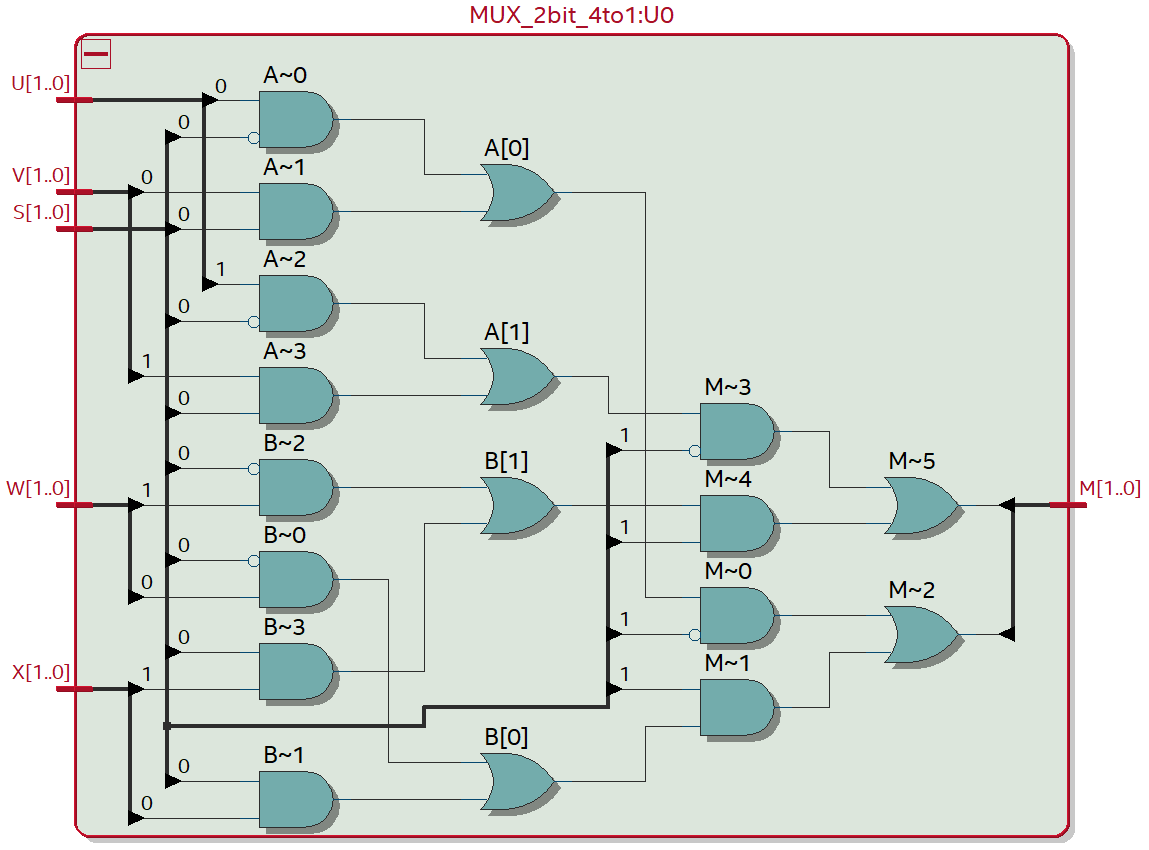
\includegraphics[width=1\textwidth]{Figures/Example_RTL.png}
    \caption{RTL view of a VHDL file} % Caption
    \label{fig:mux} % Label is used to reference later
\end{figure}

\clearpage

%inserting a subfigure, with two images underneath eachother
\begin{figure}[h]
    \centering
    \begin{subfigure}{1\textwidth} % 1\textwidth makes the subfigure size as wide as the text
        \centering
        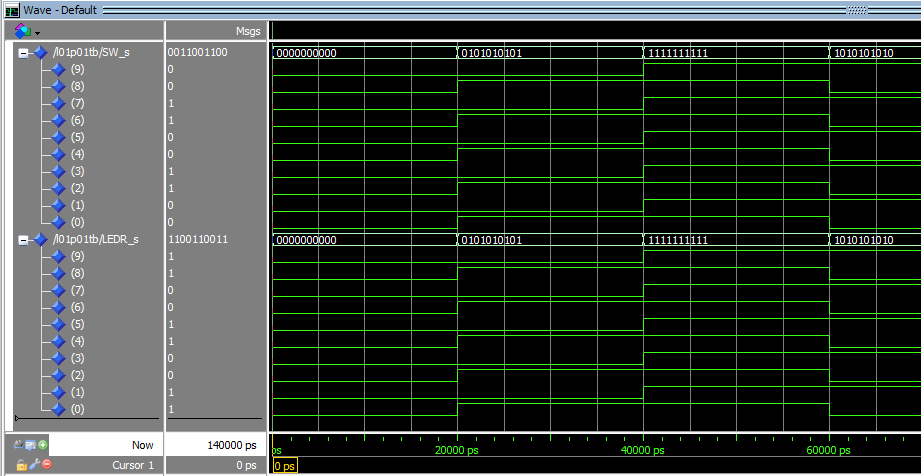
\includegraphics[width=1\textwidth]{Figures/Example_sim.png}
        \caption{First subfigure, simulation}
        \label{fig:sim_a}
    \end{subfigure}
    \begin{subfigure}{1\textwidth}
        \centering
        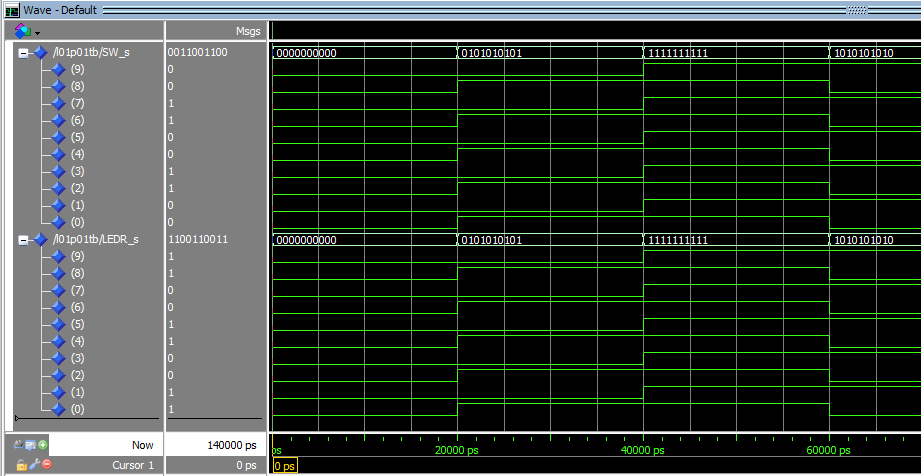
\includegraphics[width=1\textwidth]{Figures/Example_sim.png}
        \caption{Second subfigure, yes the same picture}
        \label{fig:sim_b}
    \end{subfigure}
    \caption{Simulation results, doubled up}
    \label{fig:sim}
\end{figure}

\clearpage

\begin{figure}[h]
    \centering
    \begin{subfigure}{0.45\textwidth} % 0.45\textwidth makes the subfigure under half the text width
        \centering
        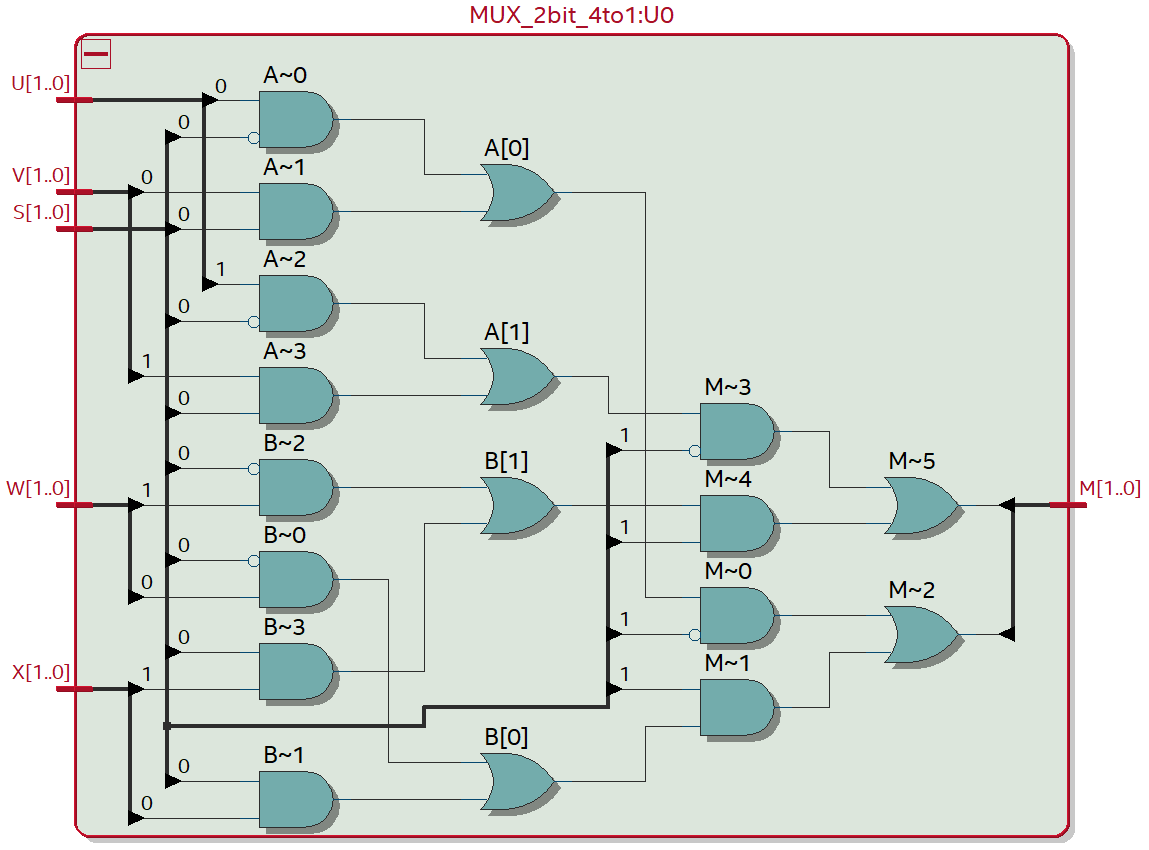
\includegraphics[width=1\textwidth]{Figures/Example_RTL.png}
        \caption{A small picture}
        \label{fig:miniRTL1}
    \end{subfigure}
    \hfill % Using \hfill between two figures that is less than text width makes them side by side
    \begin{subfigure}{0.45\textwidth}
        \centering
        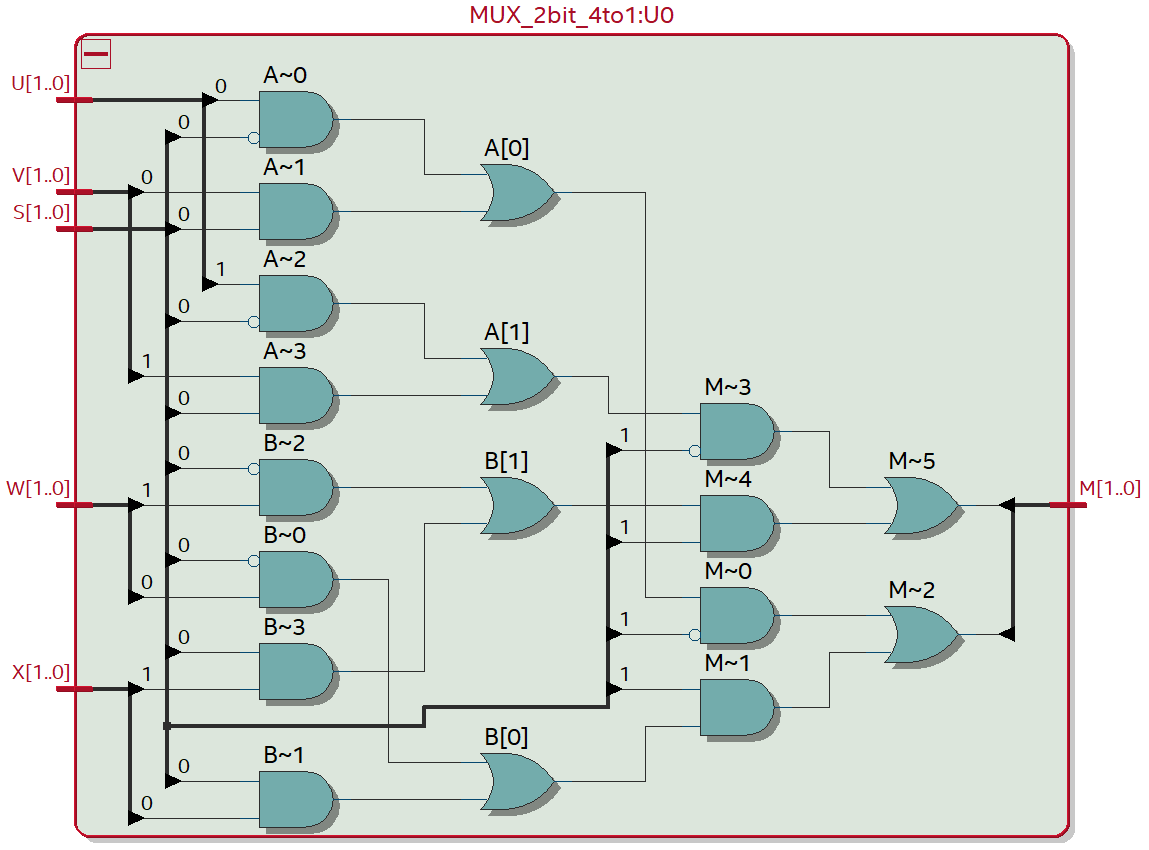
\includegraphics[width=1\textwidth]{Figures/Example_RTL.png}
        \caption{Beside another}
        \label{fig:miniRTL2}
    \end{subfigure}
    \begin{subfigure}{1\textwidth} % This is 1\textwidth so it will be underneath and wide
        \centering
        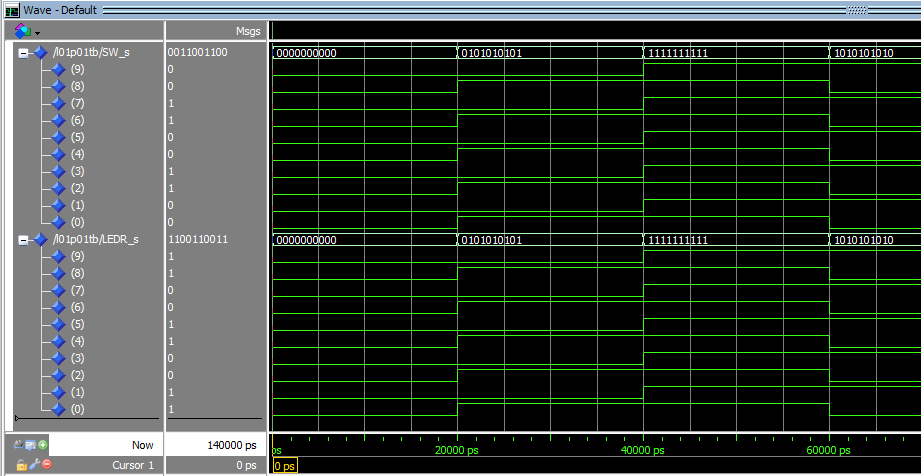
\includegraphics[width=1\textwidth]{Figures/Example_sim.png}
        \caption{And a big underneath}
        \label{fig:simUnder}
    \end{subfigure}
    \caption{All results combined together}
    \label{fig:multifig}
\end{figure}


\section{Referencing}
In this section we will reference the figures in this code and linking them.

\subsection{In document linking}
To start with you can reference the figures like Code:~\ref{Code:Example1.vhd} or Figure:~\ref{fig:mux}. This will also link them so you can click on the pdf/render and it will jump to the figure.\\ % the \\ means new paragraph
Note, figures work well, with this as clicking the link brings you to the top of the figure, for codes you get to the bottom/caption instead. This is due to the way captions is added to the code blocks to keep them working for multipage blocks.
% Code blocks get the automatic label as Code:filename, and figures you set the label yourself
% Worth mentioning that keeping the naming convention clean is a good idea, also figure numbering
% is automatic and it is best to not use numbering in lables except for diffenecing versions of
% similar figures, like fig:mux1 and fig:mux2 or as a descriptive nature fig:8bitsystem.

\subsection{websites}
For referencing external link like a URL. there are two ways \url{www.example.com} makes all of it visible, best for printing, if you want an embedded link in text \href{www.example.com}{do like this}. You can see by clicking it both should lead to the same website.

\end{document}
